\section * {Results} \label{sec:results}

\begin{sidewaysfigure} \label{fig:results1}
	\centering
	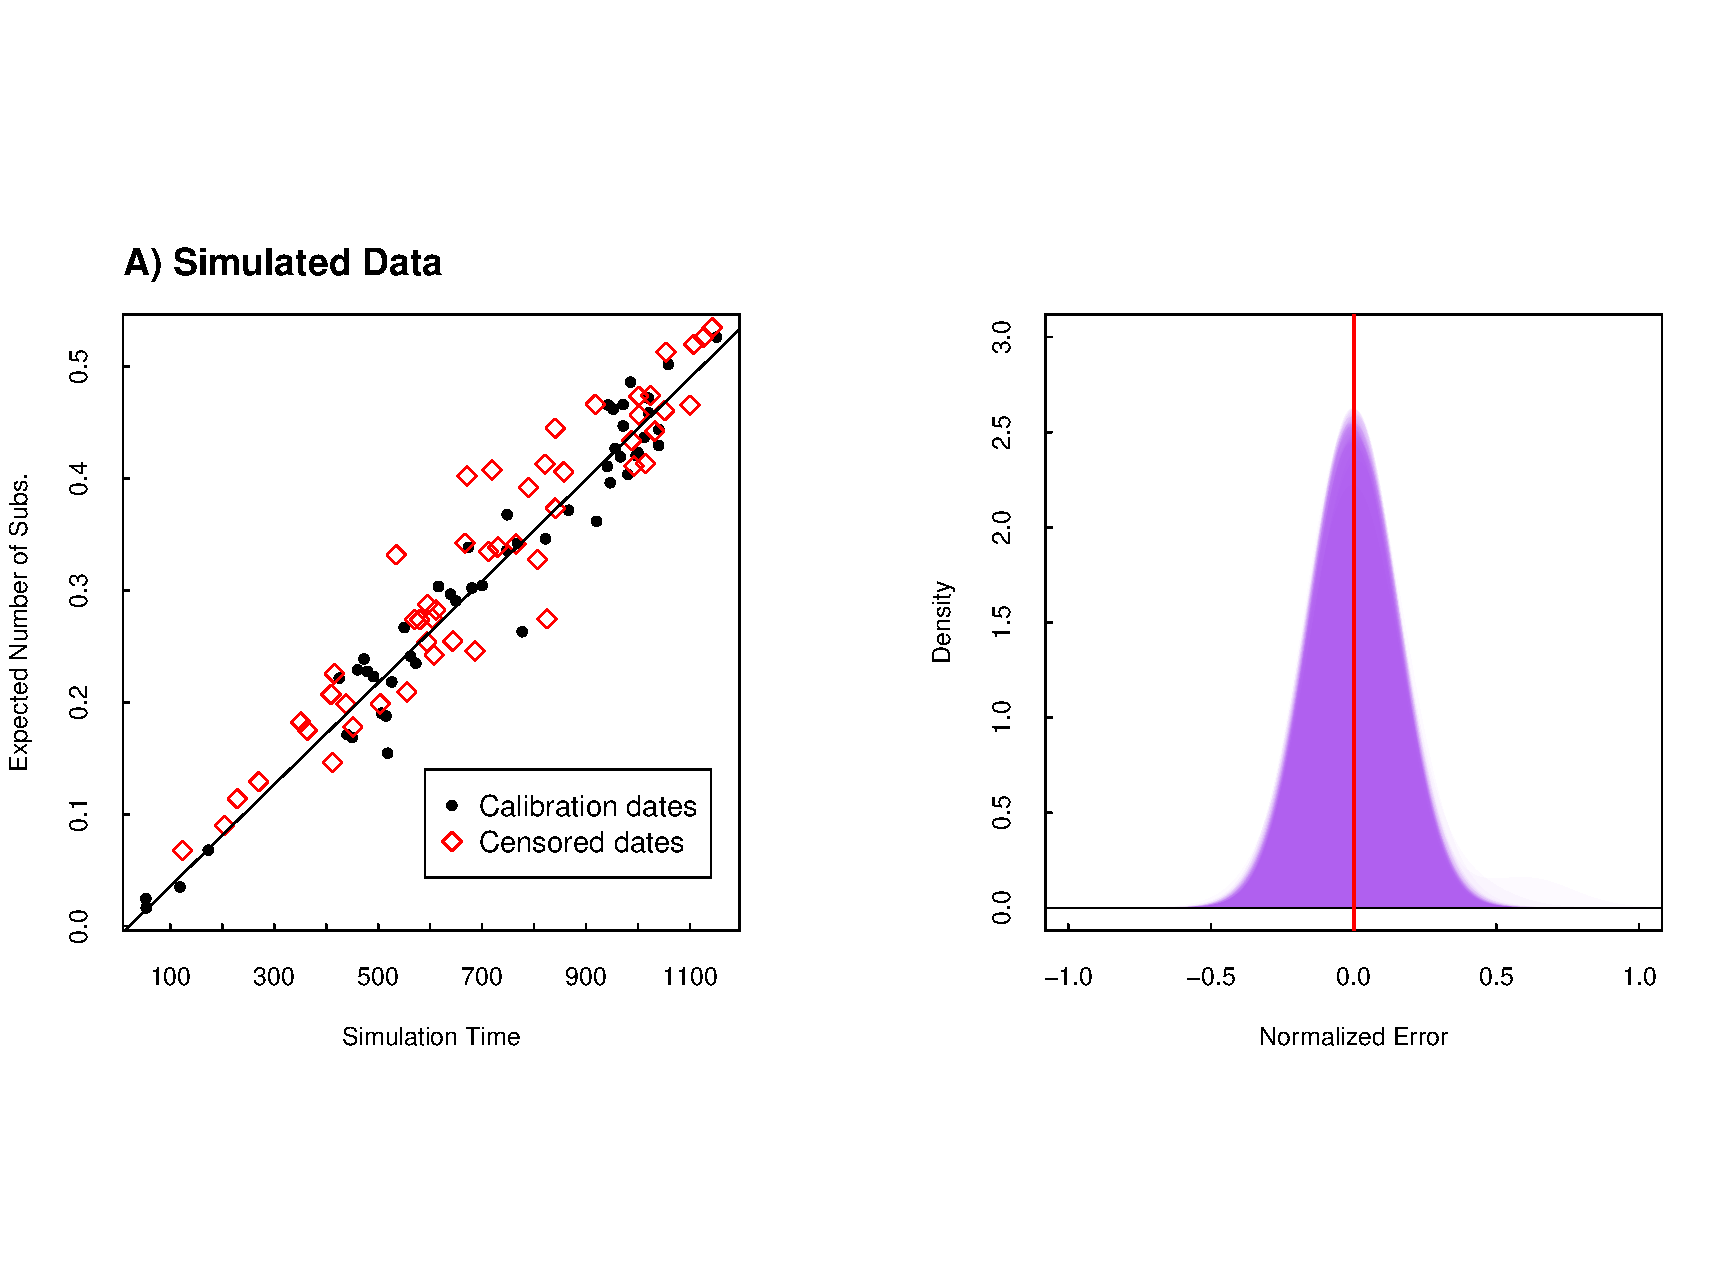
\includegraphics[trim=0cm 0cm 0cm 6cm, clip=true, scale=0.425]{figures/simulated.pdf} \\
	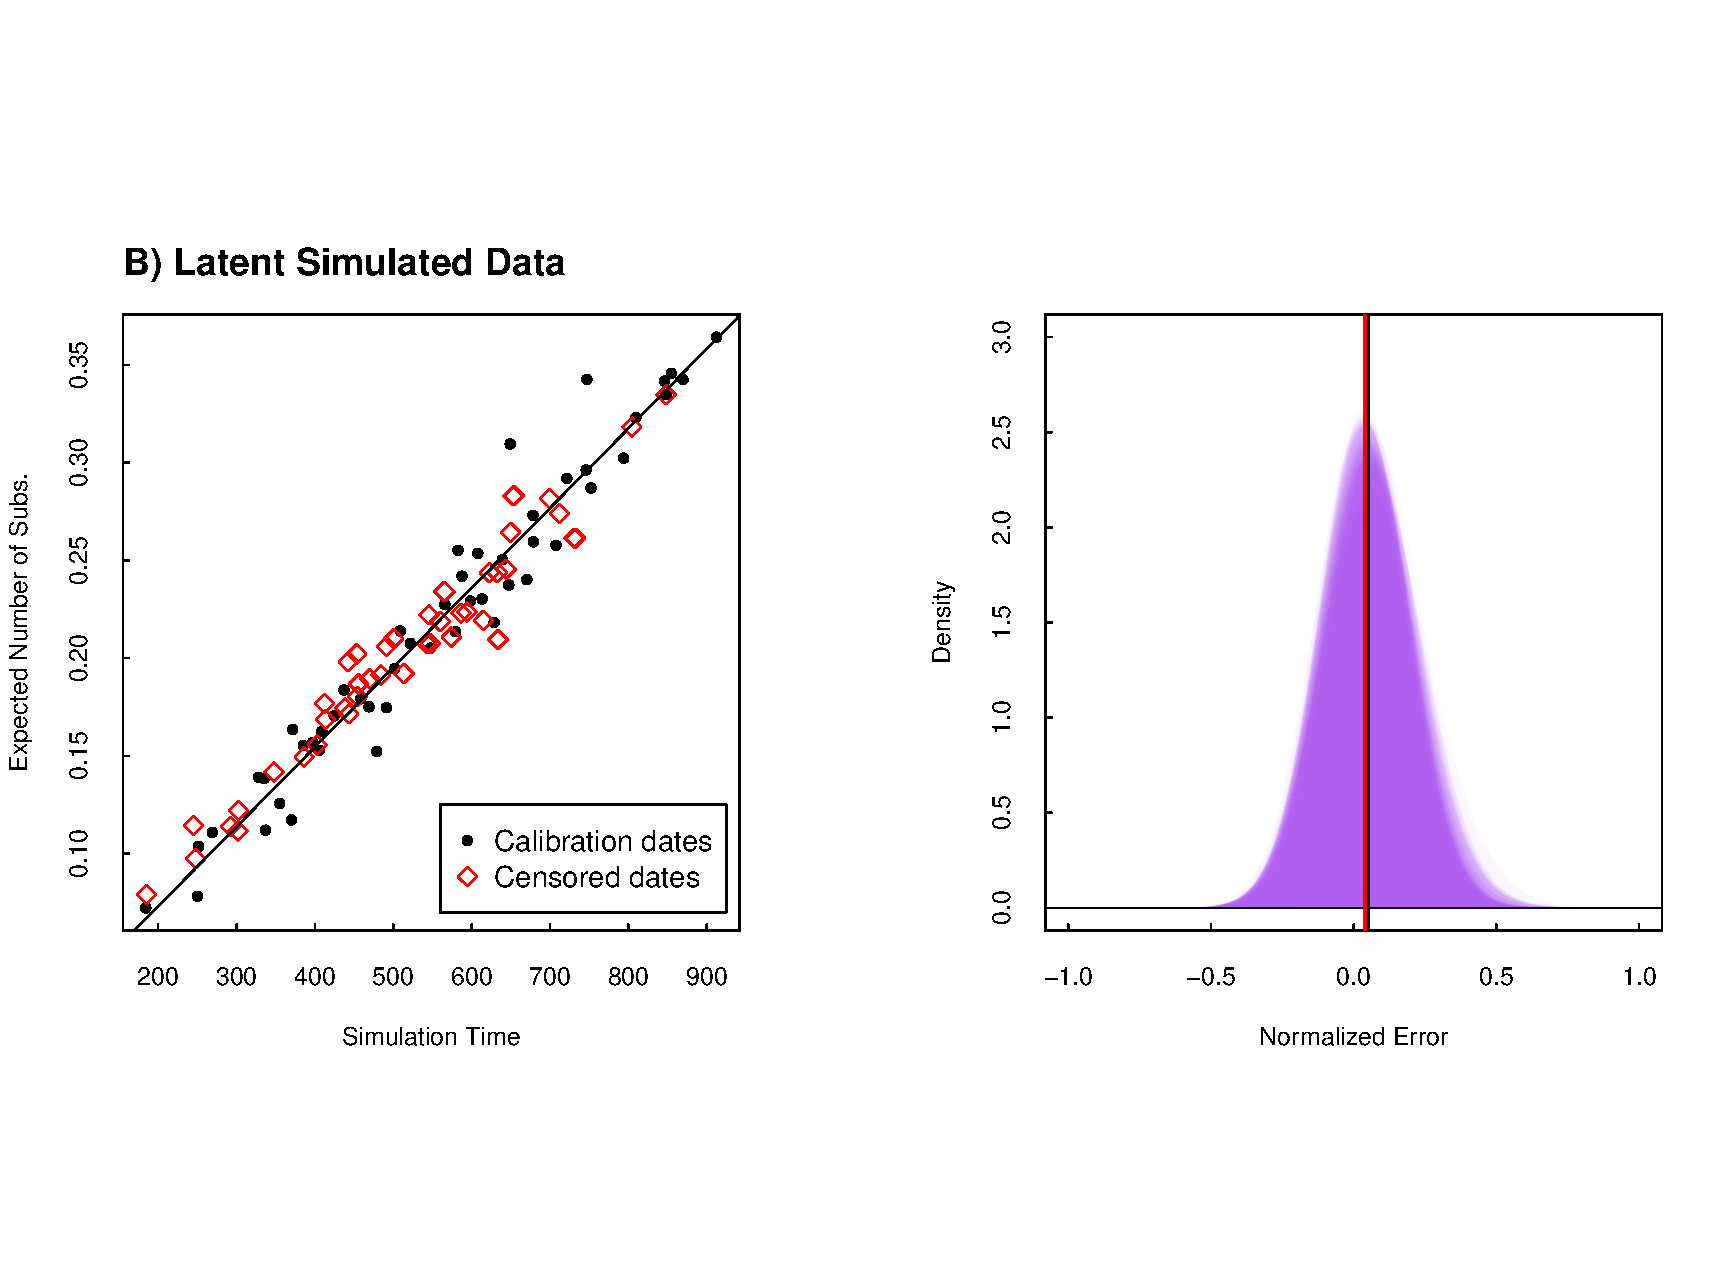
\includegraphics[trim=0cm 0cm 0cm 7cm, clip=true,scale=0.425]{figures/simulated_latent.pdf}\\
	\caption[Simulated Data]{On the left of each case is a plot of evolutionary distance vs time, the right is a the super position of density estimates (of normalized error) for each phylogeny (with kernel bandwidth = $0.15$). The red line on the density plot is the mean error, and the black line is the median error. }
\end{sidewaysfigure}

\begin{sidewaysfigure} \label{fig:results2}
	\centering
	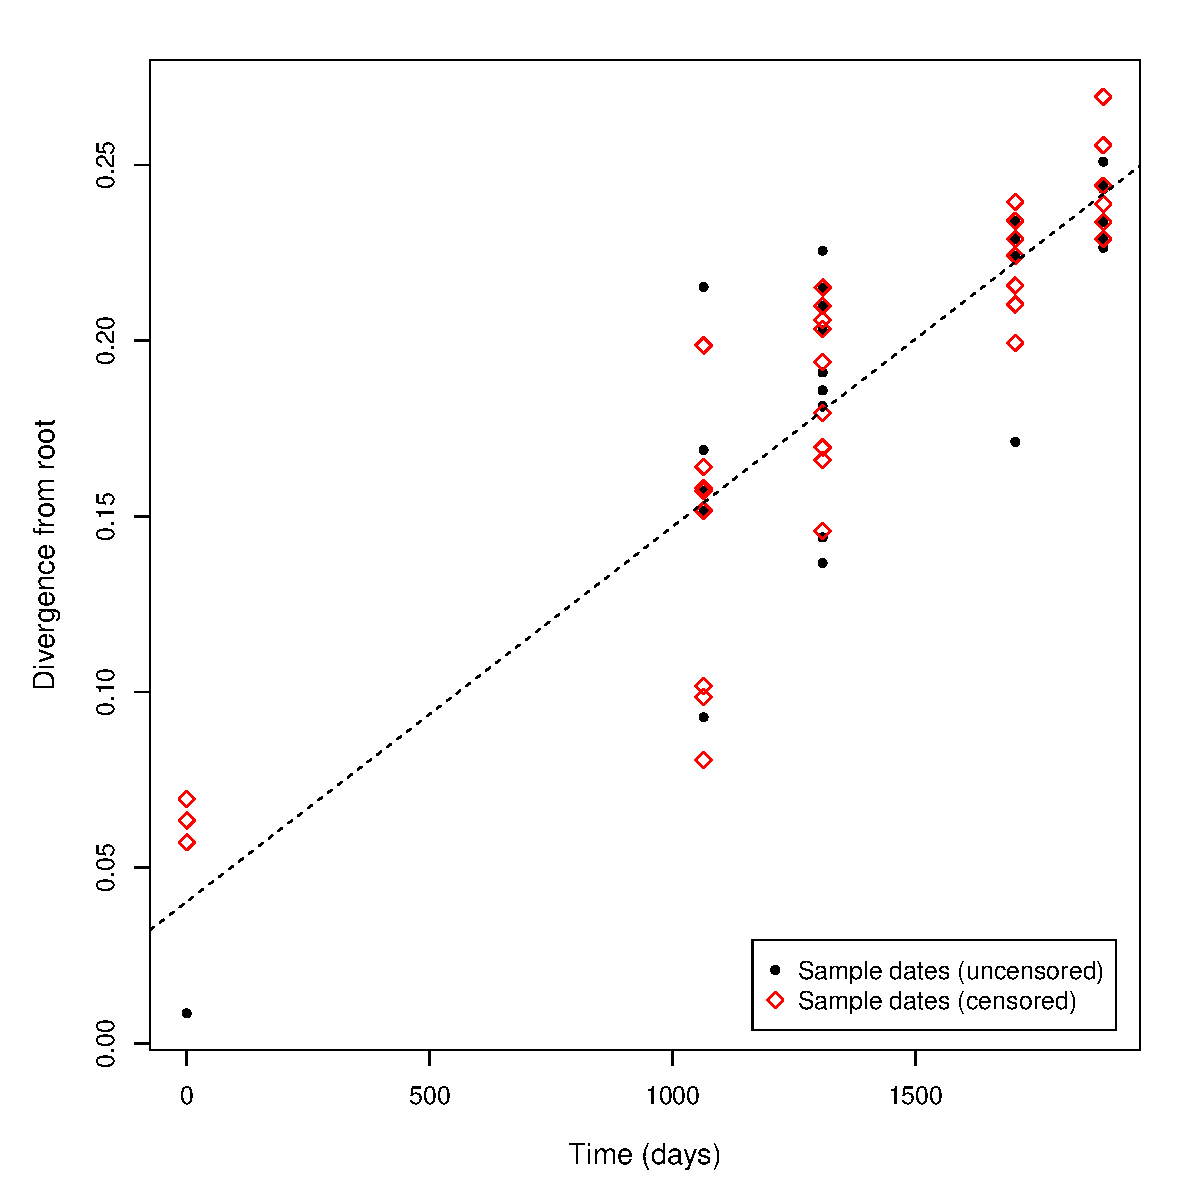
\includegraphics[trim=0cm 0cm 0cm 7cm, clip=true,scale=0.425]{figures/ancre.pdf}\\
	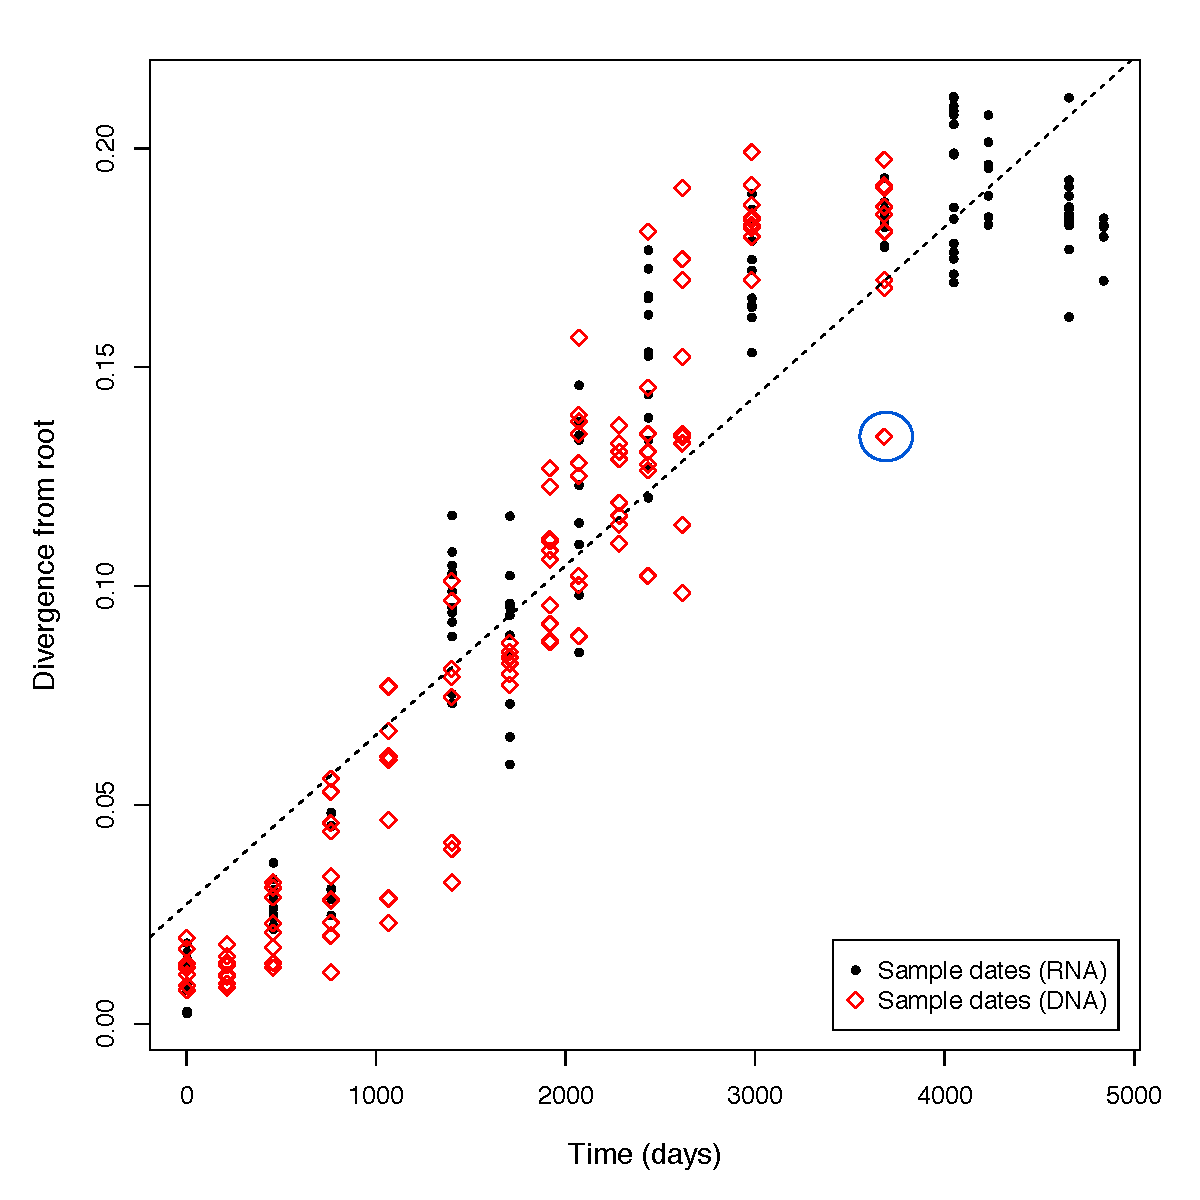
\includegraphics[trim=0cm 4cm 0cm 7cm, clip=true,scale=0.425]{figures/lanl.pdf}
	\caption[Examples]{This figure is as the previous, except for the real data.
The phylogenies in these cases have been rooted with outgroup rooting}
\end{sidewaysfigure}


\subsection * {Model Validation} \label{sec:sim_results}
Figure \ref{fig:results1} shows our model validation results over our synthetic data -- here we censor 50\% of the dates, and attempt to reconstruct them. 
Under the assumption of a strict molecular clock (that evolution is linearly related to time) the clock is a reliable source of information for these simulations.
Figure \ref{fig:results1} A shows this result for the synthetic data with no latent behaviour.
Averaged over all simulated data sets, the mean square error was $3.0\times 10^{-3}$, and the average median and mean difference were 0 and $5.0\times 10^{-5}$ respectively. 
Quantitatively, the censored data points are close to the regression line, and the difference density is heavily peaked around 0. 

Figure \ref{fig:results1} B shows different results for the latent simulations -- here we censor 50\% of the dates, attempt to reconstruct them, then compare them to the simulated collection dates. 
In this case, averaged over all simulated data sets, the mean square error was $7.1\times 10^{-3}$, and the average median and mean difference were $4.0\times 10^{-2}$ and $5.1\times 10^{-2}$ respectively. 
This bias is expected, as the errors were calculated between the simulated collection times -- not the simulated archival times.
More quantitatively, we expect the density plot to be shifted to the right (as it is in figure \ref{fig:results1} B) as this suggests that sequences are older than their sampling dates.
When we performed the same analysis against the simulated archival times, the results were nearly identical to the results without any latent data, suggesting that we can recover the dates of latent sequences provided an accurate clock.

For our final validation, we took the same strategy as the first validation on synthetic data, and applied it to our {\em plasma} data set -- we censored known sampling dates, then attempted to reconstruct them (Figure \ref{fig:results2} C shows this when the phylogenies have been rooted with outgroup rooting). 
Averaged over all simulated data sets, the mean square error was $1.7\times 10^{-1}$, and the absolute value of average median and mean difference were $2.1\times 10^{-4}$ and $1.9\times 10^{-2}$ respectively. 
The density plot shows similar behavior to that of the synthetic data, except with a wider distribution, and more variation. 

\subsection * {Application} \label{sec:mixed_data}

Finally, we tested our methodology on the {\em mixed} data set.
Figure \ref{fig:results2} D shows the regression over the plasma calibration dates the plasma collection dates. 
In this case, we do not know the actual date of archival, however, the superposition of the difference density plots shows similar behavior to that of the latent simulated data.

With respect to the sampling time, over all individuals, the mean square error was $4.9\times 10^{-2}$, and the absolute value of average median and mean difference were $2.4\times 10^{-2}$ and $4.7\times 10^{-3}$.

Individuals that had received treatment at some point generally failed the hypothesis test -- there was only one patient that did not -- these individuals were not included in the above analysis. 

